\documentclass{article}

% if you need to pass options to natbib, use, e.g.: \PassOptionsToPackage{numbers, compress}{natbib} before loading
%     neurips_2020

% ready for submission \usepackage{neurips_2020}

% to compile a preprint version, e.g., for submission to arXiv, add add the [preprint] option:
% \usepackage[preprint]{neurips_2020}

% to compile a camera-ready version, add the [final] option, e.g.: \usepackage[final]{neurips_2020}

\PassOptionsToPackage{numbers, compress}{natbib}

% to avoid loading the natbib package, add option nonatbib:
     \usepackage[preprint]{neurips_2020}

\usepackage[utf8]{inputenc} % allow utf-8 input
\usepackage[T1]{fontenc}    % use 8-bit T1 fonts
\usepackage{hyperref}       % hyperlinks
\usepackage{url}            % simple URL typesetting
\usepackage{booktabs}       % professional-quality tables
\usepackage{amsfonts}       % blackboard math symbols
\usepackage{amsmath}
\usepackage{nicefrac}       % compact symbols for 1/2, etc.
\usepackage{microtype}      % microtypography
\usepackage{listings}
\usepackage{graphicx}
\usepackage{caption}
\usepackage{subcaption}

\title{Semantic segmentation using full convolutional network}

% The \author macro works with any number of authors. There are two commands used to separate the names and addresses of
% multiple authors: \And and \AND.
%
% Using \And between authors leaves it to LaTeX to determine where to break the lines. Using \AND forces a line break at
% that point. So, if LaTeX puts 3 of 4 authors names on the first line, and the last on the second line, try using \AND
% instead of \And before the third author name.

\author{%
  Fangzhou Ai\\
  Department of Electrical and Computer Engineering\\
  University of California, San Diego\\
  La Jolla, CA 92093 \\
  \texttt{faai@eng.ucsd.edu} \\
  % examples of more authors
   \And Yue Qiao \\
   Department of Electrical and Computer Engineering \\
   University of California, San Diego\\
   La Jolla, CA 92093 \\
   \texttt{yuq021@eng.ucsd.edu}\\
   \And Zunming Zhang \\
   Department of Electrical and Computer Engineering \\
   University of California, San Diego\\
   La Jolla, CA 92093 \\
   \texttt{zuz008@eng.ucsd.edu}\\
}

\begin{document}

\maketitle

\begin{abstract}
  In this report, we explore the full convolutional network (fcn) and use full convolutional network to perform semantic
  segmentation task on Indian driving dataset. Using our baseline dataset, we archive pixel accuracy of $0.79$ and
  average IOU of $0.33$.
\end{abstract}

%--------------------------------------------

\section{Introduction}

In the report we try to solve the sematic segmentation task using full convolutional network. The goal of semantic
segmentation is to label each pixel of an image with a corresponding class of what is being represented
\cite{Anovervi90:online}. To solve the task, we utilize full convolutional network. In full convolutional network, there
is no fully connected layer, only convolutional layer. In the full convolutional network structure, we use Xavier weight
initialization. Deep neural network suffers from weight vanishing problem. If we use normal weight initialization
methods like uniform distribution, the weight will vanish quickly during matrix calculation. Therefore, we introduces
Xavier weight initialization \cite{pmlr-v9-glorot10a}, which can help us eliminate the problem. To further improve the
training speed and stability of the network, we introduce batch normalization layer \cite{ioffe2015batch}. The batch
normalization layer solves that the distribution of each layer's inputs changes during training by normalizing layer
inputs.

%--------------------------------------------

\section{Related Work}

%--------------------------------------------

\section{Methods}

\subsection{Baseline}

The baseline model is an encoder-decoder structure. It first encode the picture using convolution layers and then decode
the segmentation map using deconvolution layers. In the baseline model, we use batch normalization and use ReLU as the
activation function. For the last layer, we use softmax to get the classify results.

\subsection{Improved baseline}

\subsubsection{Dataset Augmentation}

From the baseline model, we tried to do some data augmentation on the training dataset to see whether the performance
could be approved. Since training is quite time-consuming, in this report, we implemented and tested two different data
augmentation algorithm and tried to compare the performance with each other.

The data augmentation methods used are:
\begin{itemize}
  \item Mirror flip: for the training dataset, we mirror flipped the dataset and fed them into the model
  \item Image Rotating: rotate the images slightly (for a certain degree), in this report, we tried to rotate the images
        by 1 degree and then fed them into the model
\end{itemize}

\subsubsection{Imbalanced class problem}

For the imbalanced class problem, what we usually do is to pressuring the network to categorize the infrequently seen
class. We proposed to use the weighted loss method to accommodate this issue, which will weight infrequent classes more.

For the weighted loss, the idea is to set the weight of the loss of each class inversely proportion to the frequency of
each class in the training dataset. For the data pre-processing, we calculated the total pixel count of each class in
all the training dataset and then use this information to help us set the weight of the loss.

Suppose, the number of samples for each class is stored in nSamples, then we use $\text{normedWeights} = [1 - (x /
  \sum\text{nSamples}) \text{ for } x \text{ in} \text{ nSamples}]$ as the normalized weight of the loss for each class.

For this dataset, we calculated the number of samples for each class is:

$ \text{nSamples} = [2198453584,519609102,28929892,126362539,58804972,59032134, $

$ 94293190,2569952,101519794,163659019,105075839,47400301,30998126,133835645, $

$ 135950687,41339482,15989829,104795610,8062798,450973,94820222,341805135, $

$557016609,71159311,1465165566,1823922767,2775322]$

Then we could be able to set the weight of the loss for each class according to nSamples.

\subsection{Custom model}

Inspired by this paper\cite{alom2018recurrent}, we replace the encoder part in FCN model with the RRCNN layer instead,
the RRCNN represent better abstraction ability, thus we would expect better IoU and precision. However the RRCNN is
really memory-intensive, we have to crop the image to only 256 *256 size and delete 3 layers from original model's
encoding part, which severly influence the performance of our model. What's worse is the RRCNN encoding part contains
maxpooling operation after each RRCNN block, which means the images size would shrinks even more, since we have already
started from a relative small size, maxpool will almost ruin all the details in the feature map.

\subsection{Transfer learning}

In this part we employ the DEEPLABV3-RESNET101 model, which is a default pre-trained net work in PyTorch, from the
website\cite{Deeplabv74:online} we know that this model is constructed by a Deeplabv3 model with a ResNet-101 backbone.
The pre-trained model has been trained on a subset of COCO train2017, on the 20 categories that are present in the
Pascal VOC dataset. We modifier the classifier part so that it could match the number of our feature, and we freeze the
parameters of the pretrained part to accelerate the whole procedure.

\subsection{U-Net}

Folowing the routine demostrated in the U-net paper \cite{ronneberger2015unet}, we build the U-net by our self. The
obvious difference is the U-net convolution block contains 2 convolution of the same size, while the FCN model only
contains 1 convolution operation. We notice that the U-net model is also memory intensive while the datahub only give us
a GTX 1080 ti with  11GB memory, hence there's a trade-off of between batch size, image size and model's completeness.
We decide to crop the image and shrink the batch size to run the whole model, though this might not be the best
solution, but this could give us a flavor of how the complete network looks like.

%--------------------------------------------

\section{Results}

\begin{table}[h]
  \caption{Pixel accuracy and IOUs for different models}
  \label{table:results}
  \centering
  \hspace*{-1.2cm}\begin{tabular}{@{}llllllll@{}}
    \toprule
    Model             & Pixel accuracy & Mean IOU & road IOU & sidewalk IOU & car IOU & billboard IOU & sky IOU \\
    \midrule Baseline & 0.7944         & 0.3371   & 0.8632   & 0.2323       & 0.5084  & 0.2419        & 0.9403
    \\
    Mirror flip       & 0.6953         & 0.2313   & 0.7477   & 0.0874       & 0.2262  & 0.2542        & 0.8105  \\
    Rotation          & 0.7936         & 0.3393   & 0.8577   & 0.2483       & 0.4857  & 0.2755        & 0.9445  \\
    weighted loss     & 0.7991         & 0.3444   & 0.8648   & 0.2406       & 0.5104  & 0.2967        & 0.9472  \\
    Custom            & TBA            & TBA      & TBA      & TBA          & TBA     & TBA           & TBA     \\
    Transfer learning & TBA            & TBA      & TBA      & TBA          & TBA     & TBA           & TBA     \\
    U-Net             & TBA            & TBA      & TBA      & TBA          & TBA     & TBA           & TBA
    \\\bottomrule
  \end{tabular}
\end{table}

Training and Validation loss for baseline model is in \autoref{fig:loss_train_val_baseline}. Training and Validation
pixel accuracy and mean IOUs for baseline model is in \autoref{fig:pixel_accuracy_mean_iou_val_baseline}. Various IOUs
for baseline model is in \autoref{fig:various_iou_val_baseline}.

\begin{figure}[h]
  \centering
  \begin{subfigure}[b]{0.49\textwidth}
    \centering
    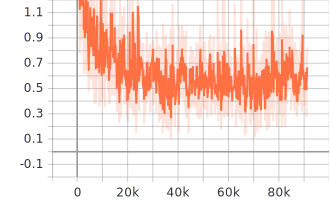
\includegraphics[width=\textwidth]{Loss_train_baseline.png}
    \caption{Training loss}
    \label{fig:loss_train_baseline}
  \end{subfigure}
  \hfill
  \begin{subfigure}[b]{0.49\textwidth}
    \centering
    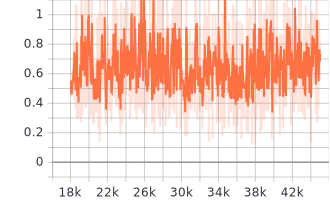
\includegraphics[width=\textwidth]{Loss_val_baseline.png}
    \caption{Validation loss}
    \label{fig:loss_val_baseline}
  \end{subfigure}
  \caption{Training and Validation loss for baseline model}
  \label{fig:loss_train_val_baseline}
\end{figure}

\begin{figure}[h]
  \centering
  \begin{subfigure}[b]{0.49\textwidth}
    \centering
    \includegraphics[width=\textwidth]{Pixel Accuracy_Val_baseline.png}
    \caption{Pixel accuracy}
    \label{fig:pixel_accuracy_val_baseline}
  \end{subfigure}
  \hfill
  \begin{subfigure}[b]{0.49\textwidth}
    \centering
    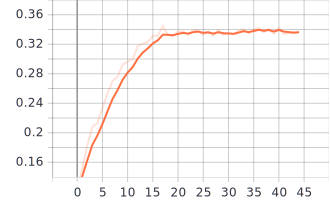
\includegraphics[width=\textwidth]{IOU_Average_Val_baseline.png}
    \caption{Mean IOUs}
    \label{fig:mean_iou_val_baseline}
  \end{subfigure}
  \caption{Training and Validation pixel accuracy and mean IOUs for baseline model}
  \label{fig:pixel_accuracy_mean_iou_val_baseline}
\end{figure}

\begin{figure}[h]
  \centering
  \begin{subfigure}[b]{0.19\textwidth}
    \centering
    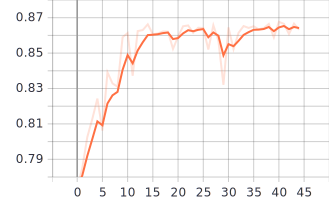
\includegraphics[width=\textwidth]{IOU_Road_Val_baseline.png}
    \caption{Road IOU}
    \label{fig:road_iou_val_baseline}
  \end{subfigure}
  \hfill
  \begin{subfigure}[b]{0.19\textwidth}
    \centering
    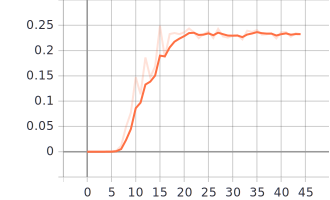
\includegraphics[width=\textwidth]{IOU_Sidewalk_Val_baseline.png}
    \caption{Sidewalk IOU}
    \label{fig:sidewalk_iou_val_baseline}
  \end{subfigure}
  \hfill
  \begin{subfigure}[b]{0.19\textwidth}
    \centering
    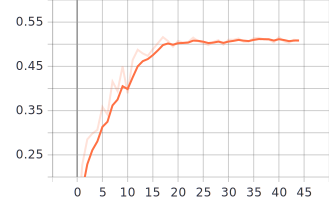
\includegraphics[width=\textwidth]{IOU_Car_Val_baseline.png}
    \caption{Car IOU}
    \label{fig:car_iou_val_baseline}
  \end{subfigure}
  \hfill
  \begin{subfigure}[b]{0.19\textwidth}
    \centering
    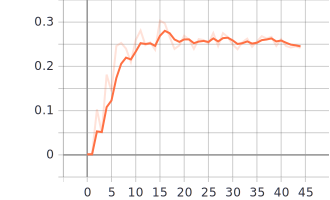
\includegraphics[width=\textwidth]{IOU_Billboard_Val_baseline.png}
    \caption{Billboard IOU}
    \label{fig:billboard_iou_val_baseline}
  \end{subfigure}
  \hfill
  \begin{subfigure}[b]{0.19\textwidth}
    \centering
    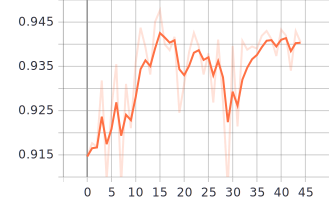
\includegraphics[width=\textwidth]{IOU_Sky_Val_baseline.png}
    \caption{Sky IOU}
    \label{fig:sky_iou_val_baseline}
  \end{subfigure}
  \caption{Various IOUs for baseline model}
  \label{fig:various_iou_val_baseline}
\end{figure}

\subsection{Improved baseline model}

\subsubsection{Dataset Augmentation}

\autoref{table:results} shows the model performance of different augmentation method. From the table, we could see
that the performance was improved by ~ 10\% simply by rotating the training dataset for a small angle.

The train and validation loss for mirror flip and rotation methods could be seen in \autoref{fig:fliploss} and
\autoref{fig:rotationloss}, respectively. The visualization of the segmented output for the first image in the test.csv
overlaid on the image for mirror flip and rotation method could be seen in \autoref{fig:mirror_flip} and
\autoref{fig:rotation}, respectively.

\begin{figure}[h]
  \centering
  \begin{subfigure}[b]{0.49\textwidth}
    \centering
    \includegraphics[width=\textwidth]{flip_loss.png}
    \caption{Training and validation loss for flip augmentation method}
    \label{fig:fliploss}
  \end{subfigure}
  \hfill
  \begin{subfigure}[b]{0.49\textwidth}
    \centering
    \includegraphics[width=\textwidth]{rotate_loss.png}
    \caption{Training and validation loss for Rotation augmentation method}
    \label{fig:rotationloss}
  \end{subfigure}
  \caption{Training and validation loss for different augmentation methods}
  \label{fig:loss_train_val_augmentation}
\end{figure}

\begin{figure}[h]
  \centering
  \begin{subfigure}[b]{0.49\textwidth}
    \centering
    \includegraphics[width=\textwidth]{flip_method.png}
    \caption{Visualization of segmented output for Mirror flip augmentation method}
    \label{fig:mirror_flip}
  \end{subfigure}
  \hfill
  \begin{subfigure}[b]{0.49\textwidth}
    \centering
    \includegraphics[width=\textwidth]{rotate_method.png}
    \caption{Visualization of segmented output for Rotation augmentation method}
    \label{fig:rotation}
  \end{subfigure}
  \caption{Visualization of segmented output for different augmentation methods}
  \label{fig:visualization_augmentation}
\end{figure}

\subsubsection{Imbalanced class problem}

The train and validation loss after introducing weighted loss method could be seen in \autoref{fig:weightedloss}. The
performance of the model could be seen in \autoref{table:results} and the visualization of the segmented output for the
first image in the testdataset overlaid on the image could be seen in \autoref{fig:visualization_weighted}

\begin{figure}[h]
  \centering
  \begin{subfigure}[b]{0.49\textwidth}
    \centering
    \includegraphics[width=\textwidth]{weighted_loss.png}
    \caption{Training and validation loss for weighted loss}
    \label{fig:weightedloss}
  \end{subfigure}
  \hfill
  \begin{subfigure}[b]{0.49\textwidth}
    \centering
    \includegraphics[width=\textwidth]{rotate_loss.png}
    \caption{Visualization of result by training with weighted loss}
    \label{fig:visualization_weighted}
  \end{subfigure}
  \caption{Weighted loss}
  \label{fig:loss_visualization_weighted}
\end{figure}


\subsection{Custom model}

\subsection{Transfer learning}

\subsection{U-Net}

%--------------------------------------------

\section{Discussion}

%--------------------------------------------

\section{Individual contributions to the project}

\paragraph{Fangzhou Ai}
Custom model, Transfer learning and U-Net model.

\paragraph{Yue Qiao}

Evaluation metrics, Dataset loading and Baseline Model.

\paragraph{Zunming Zhang}

Improved baseline model with mirror flip, rotate and weighted loss for imbalanced classes.

\bibliographystyle{plainnat}
\bibliography{bibfile}

\end{document}